\section{Metodologia}
\subsection{Diapasão em um tubo fechado}
O estudo dos harmônicos em tubos fechados foi conduzido utilizando um arranjo experimental composto por um tubo cilíndrico fechado em uma de suas extremidades, um reservatório de água com altura ajustável e um conjunto de diapasões calibrados com frequências de 256 Hz, 384 Hz e 512 Hz. O tubo foi parcialmente preenchido com água, permitindo a variação da coluna de ar em seu interior através do ajuste da altura do reservatório de água como representado na \cref{fig:diapasao}.

\begin{figure}[H]
    \centering
    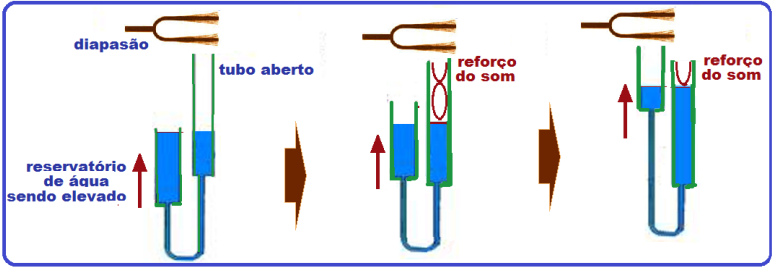
\includegraphics[width=0.50\linewidth]{fig/diapasao.png}
    \caption{Representação esquemática da montagem experimental para o estudo da ressonância em um tubo fechado. O tubo, com uma extremidade inferior fechada e parcialmente preenchido com água, permite ajustar a altura da coluna de ar por meio do nível da água, facilitando a identificação de harmônicos ao ser excitado por diapasões de diferentes frequências. Fonte: imagem fornecida pelo monitor Pedro.}
    \label{fig:diapasao}
\end{figure}

O procedimento experimental consistiu em excitar os diapasões e posicioná-los na abertura superior do tubo, perpendicularmente ao eixo longitudinal do mesmo. A altura da coluna de água foi ajustada sistematicamente até que a ressonância fosse observada.

\subsection{Ressonância e vibração em diapasão}
O arranjo experimental incluiu um diapasão de frequência fixa de 256 Hz e um segundo diapasão com frequência ajustável, equipado com um sistema de ímãs para calibração (\cref{fig:ressonancia}). A detecção da vibração no diapasão ajustável foi realizada utilizando uma pequena esfera de massa desprezível suspensa por um fio, que estava em contato com uma das hastes do diapasão.

\begin{figure}[H]
    \centering
    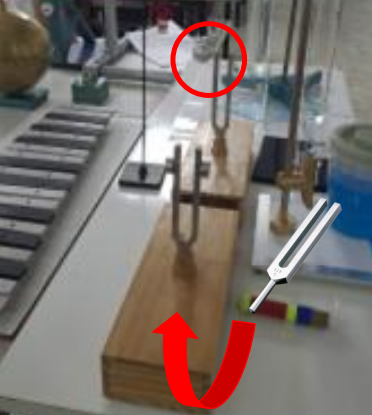
\includegraphics[width=0.25\linewidth]{fig/ressonacia.png}
    \caption{Fotografia do experimento de ressonância entre dois diapasões realizada no laboratório. O primeiro diapasão, circulado em vermelho, possui frequência fixa de 256 Hz, enquanto o segundo tem frequência ajustável por meio de ímãs. A vibração induzida é detectada por uma esfera suspensa em contato com uma das hastes do primeiro diapasão. Fonte: fotografia tirada pelo monitor Pedro}
    \label{fig:ressonancia}
\end{figure}

O procedimento iniciou-se com os dois diapasões já ajustados para a mesma frequência de 256 Hz. Em seguida, o diapasão de frequência ajustável foi percutido, e observou-se a esfera suspensa em contato com uma das hastes do primeiro diapasão. 

\subsection{Figuras de Chladni}
O estudo das figuras de Chladni foi realizado empregando duas placas metálicas planas, uma triangular e a outra quadrada, e um arco de violino (\cref{fig:chladni}). O procedimento experimental consistiu em aspergir uma fina camada de areia sobre a superfície da placa. Em seguida, a placa foi fixada em pontos estratégicos e excitada pela fricção do arco em suas bordas, gerando vibrações. Para coletar a areia que se desprendia da placa durante o experimento, um recipiente de plástico foi acoplado abaixo dos suportes das placas.

\begin{figure}[H]
    \centering
    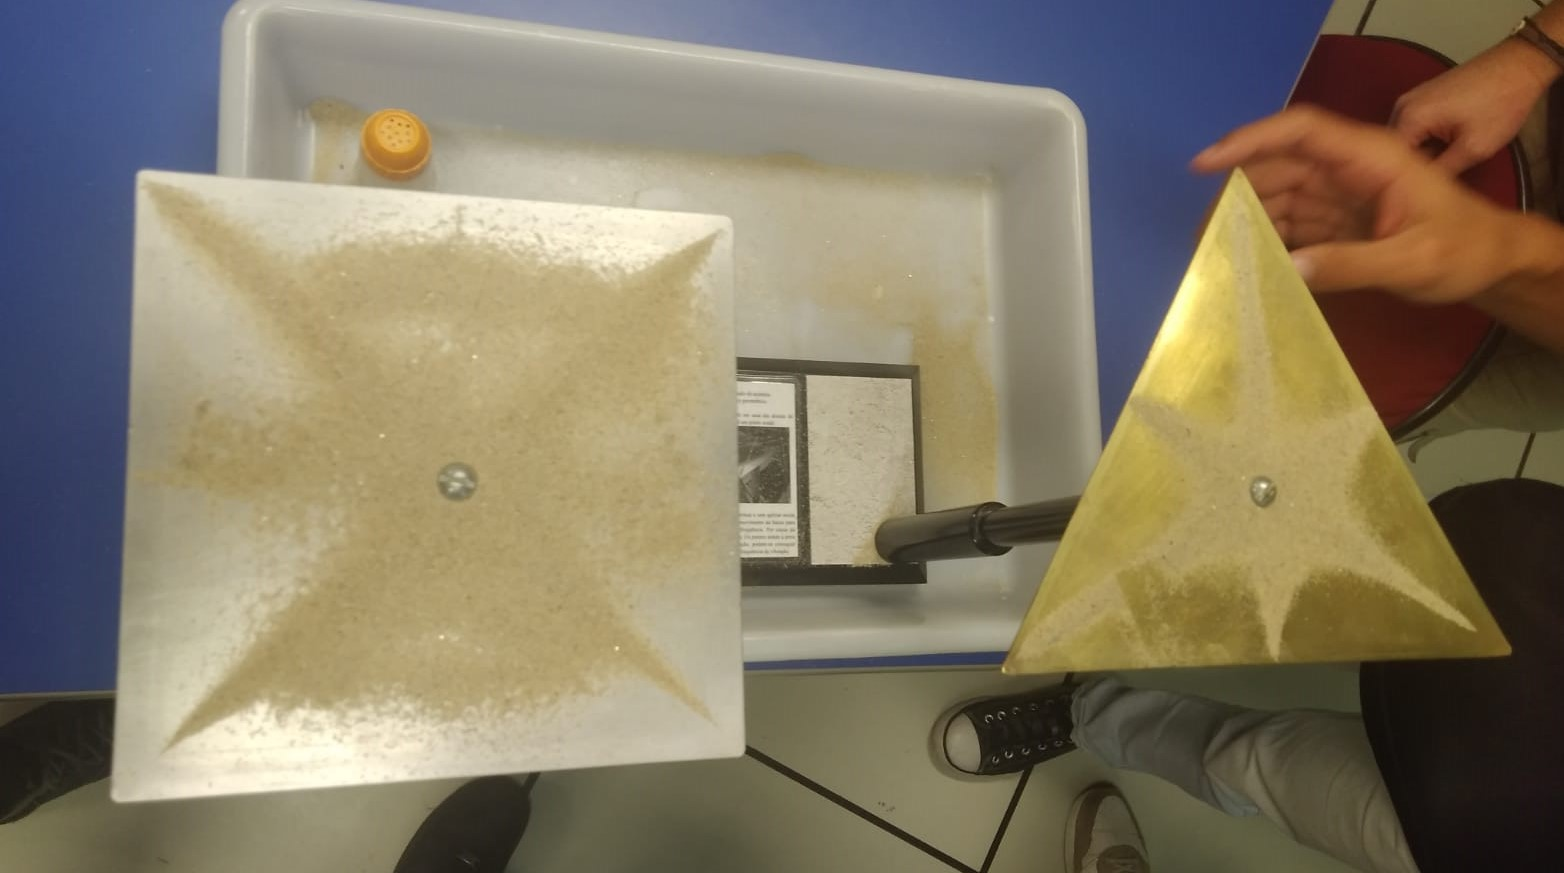
\includegraphics[width=0.35\linewidth]{fig/chladni.png.jpg}
    \caption{Fotografia tirada durante a realização do experimento de figuras de Chladni no laboratório. As placas metálicas de diferentes formas (quadrada e triangular) foram excitadas com um arco de violino, que não esta visível na imagem, formando padrões visíveis na superfície das placas. Fonte: autoria própria}
    \label{fig:chladni}
\end{figure}


Durante a experimentação, variaram-se os pontos de apoio da placa e os locais de aplicação da fricção do arco, permitindo a observação de diferentes padrões nodais formados pela areia. A análise qualitativa das figuras foi realizada para investigar a relação entre a geometria da placa, os pontos de excitação e as configurações dos padrões nodais.

\subsection{Tubo de Rijke}
O aparato experimental consistiu em um tubo cilíndrico aberto em ambas as extremidades e uma tela de malha metálica posicionada próxima a uma das extremidades do tubo. A fonte de calor de uma vela foi utilizada para aquecer a tela (\cref{fig:rijke}).

\begin{figure}[H]
    \centering
    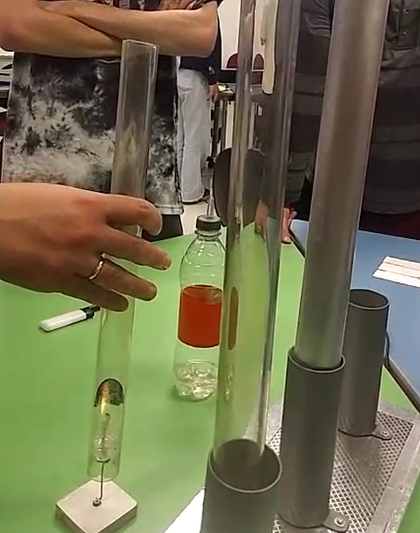
\includegraphics[width=0.25\linewidth]{fig/rijke.png}
    \caption{Registro fotográfico do experimento do tubo de Rijke feito em ambiente de laboratório. A malha metálica é aquecida por uma chama, gerando posteriormente uma emissão sonora característica quando o tubo é posicionado verticalmente. Fonte: autoria própria.}
    \label{fig:rijke}
\end{figure}

O procedimento envolveu o aquecimento inicial da tela metálica utilizando a chama da vela. Após um período de aquecimento, o tubo foi removido da chama e posicionado verticalmente. A emissão de um som característico foi observada. A influência da orientação do tubo (horizontal ou vertical) na emissão sonora foi qualitativamente investigada.

\subsection{Vibração de uma corda}
O estudo das vibrações em uma corda foi realizado utilizando um aparato que permitia variar a tensão e o comprimento efetivo da corda. O sistema incluía uma corda tensionada entre dois pontos fixos, sendo um deles móvel para ajustar o comprimento, e um mecanismo de pesos para aplicar e mensurar a tensão como mostrado na \cref{fig:umacorda}.

\begin{figure}[H]
    \centering
    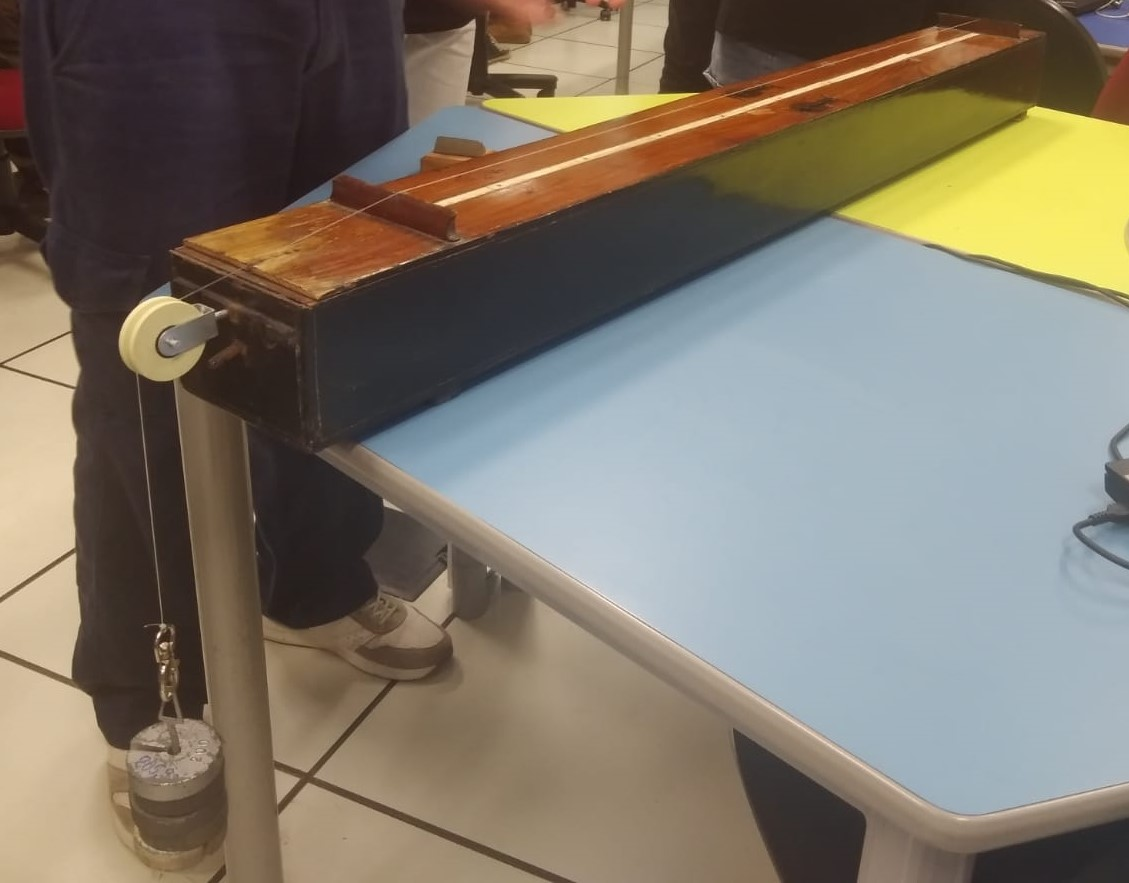
\includegraphics[width=0.30\linewidth]{fig/umacorda.png.jpg}
    \caption{Fotografia da montagem utilizada no laboratório para investigar os modos de vibração de uma corda tensionada. A tensão é aplicada com o uso de massas e o comprimento pode ser ajustado. Fonte: autoria própria.}
    \label{fig:umacorda}
\end{figure}

O experimento focou na observação dos sons gerados na corda e na relação entre a frequência de vibração, a tensão, o comprimento e a densidade linear da corda. A variação da tensão da corda e do seu comprimento efetivo foi realizada sistematicamente, e a resposta vibracional foi observada.